%!TEX root = ../main.tex

\section{Mössbauer effect}
\label{sec:mössbauer-effect}

The process of \textbf{resonant absorption} in nuclear physics describes the 
phenomenon of subsequent de- and excitation of two equal atoms to the same energy 
levels via one $\gamma$-quant. Consider for example an excited state of $^{57}$Fe,
that emits a photon with energy (roughly) \SI{14.4}{\kilo\electronvolt} during its 
transition to the ground state.

\begin{equation*}
^{57}\text{Fe}^*\;\longrightarrow\;^{57}\text{Fe}\;+\;\gamma  
\end{equation*}

In principle, one could use this emitted photon to excite another $^{57}$Fe atom to 
the higher energy state. The photon is absorbed resonantly by the second atom during 
this process.

In reality, resonant absorption such as the Na-D-line only occurs under certain
circumstances. Due to conservation laws the energy $E_\gamma$ of the emitted photon
does not exactly equal the transition energy $E_0$, but is instead shifted downward
by the nuclear recoil energy. A similar analysis finds that the energy for absorption
of the same atom is shifted upwards. 

\begin{equation}
\underbrace{E_\gamma = E_0 - \frac{p_\gamma^2}{2m}}_\text{Emission} \qquad\qquad\qquad \underbrace{E_\gamma = E_0 + \frac{p_\gamma^2}{2m}}_\text{Absorption}\label{eq:energy-gap}
\end{equation}

With the photon impulse $p_\gamma$ and atom mass $m$. If the line width introduced by
natural broadening or other effects does not exceed the energy gap, resonant 
absorption cannot occur (see \autoref{fig:resonant-absorption}). It is also notable 
that the energy gap between emission and absorption spectrum can be increased by 
additional effects. This will be further discussed in \autoref{chap:experiment}.

\begin{figure}
	\centering
	\begin{subfigure}[h]{0.45\linewidth}
	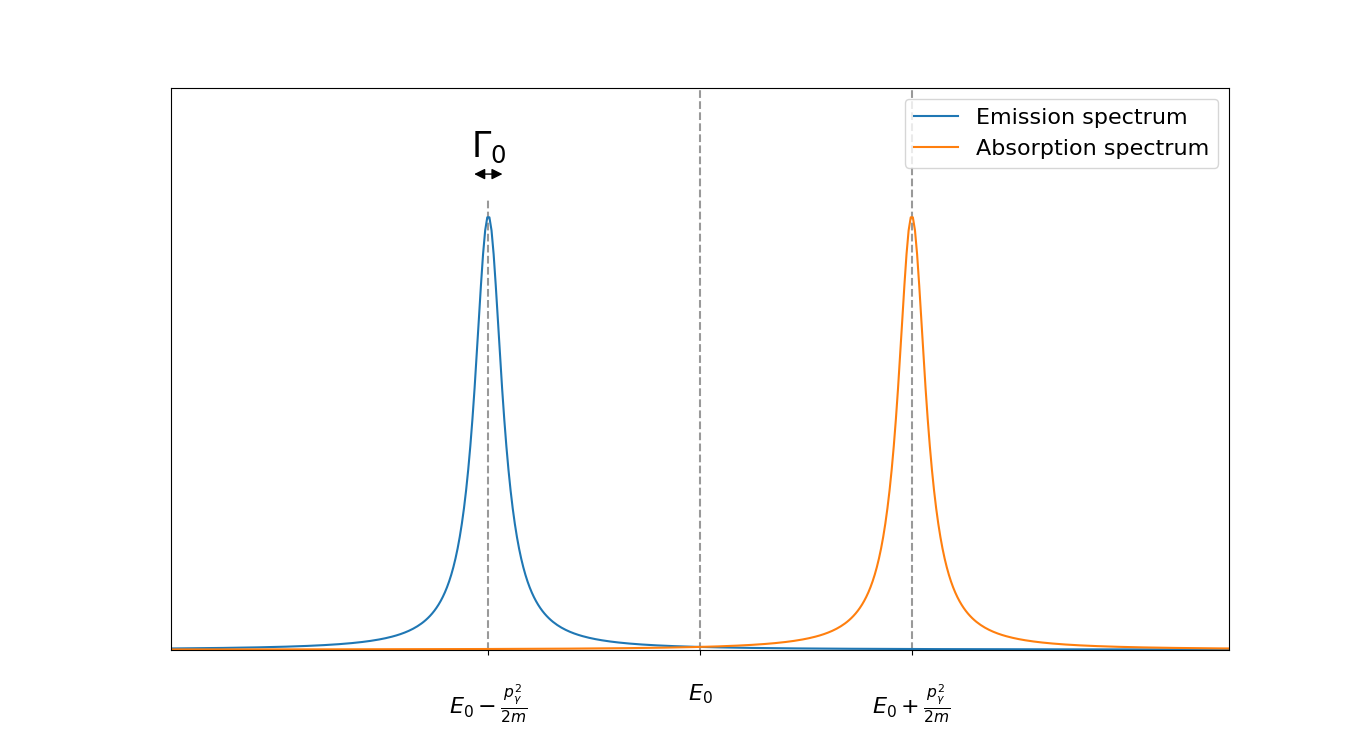
\includegraphics[height=4.0cm]{./fig/resonance-absorption-tight.png}
	\caption{\textbf{Natural broadening}\label{fig:resonance-absorption-tight}}
	\end{subfigure}
	\hfill
	\begin{subfigure}[h]{0.45\linewidth}
	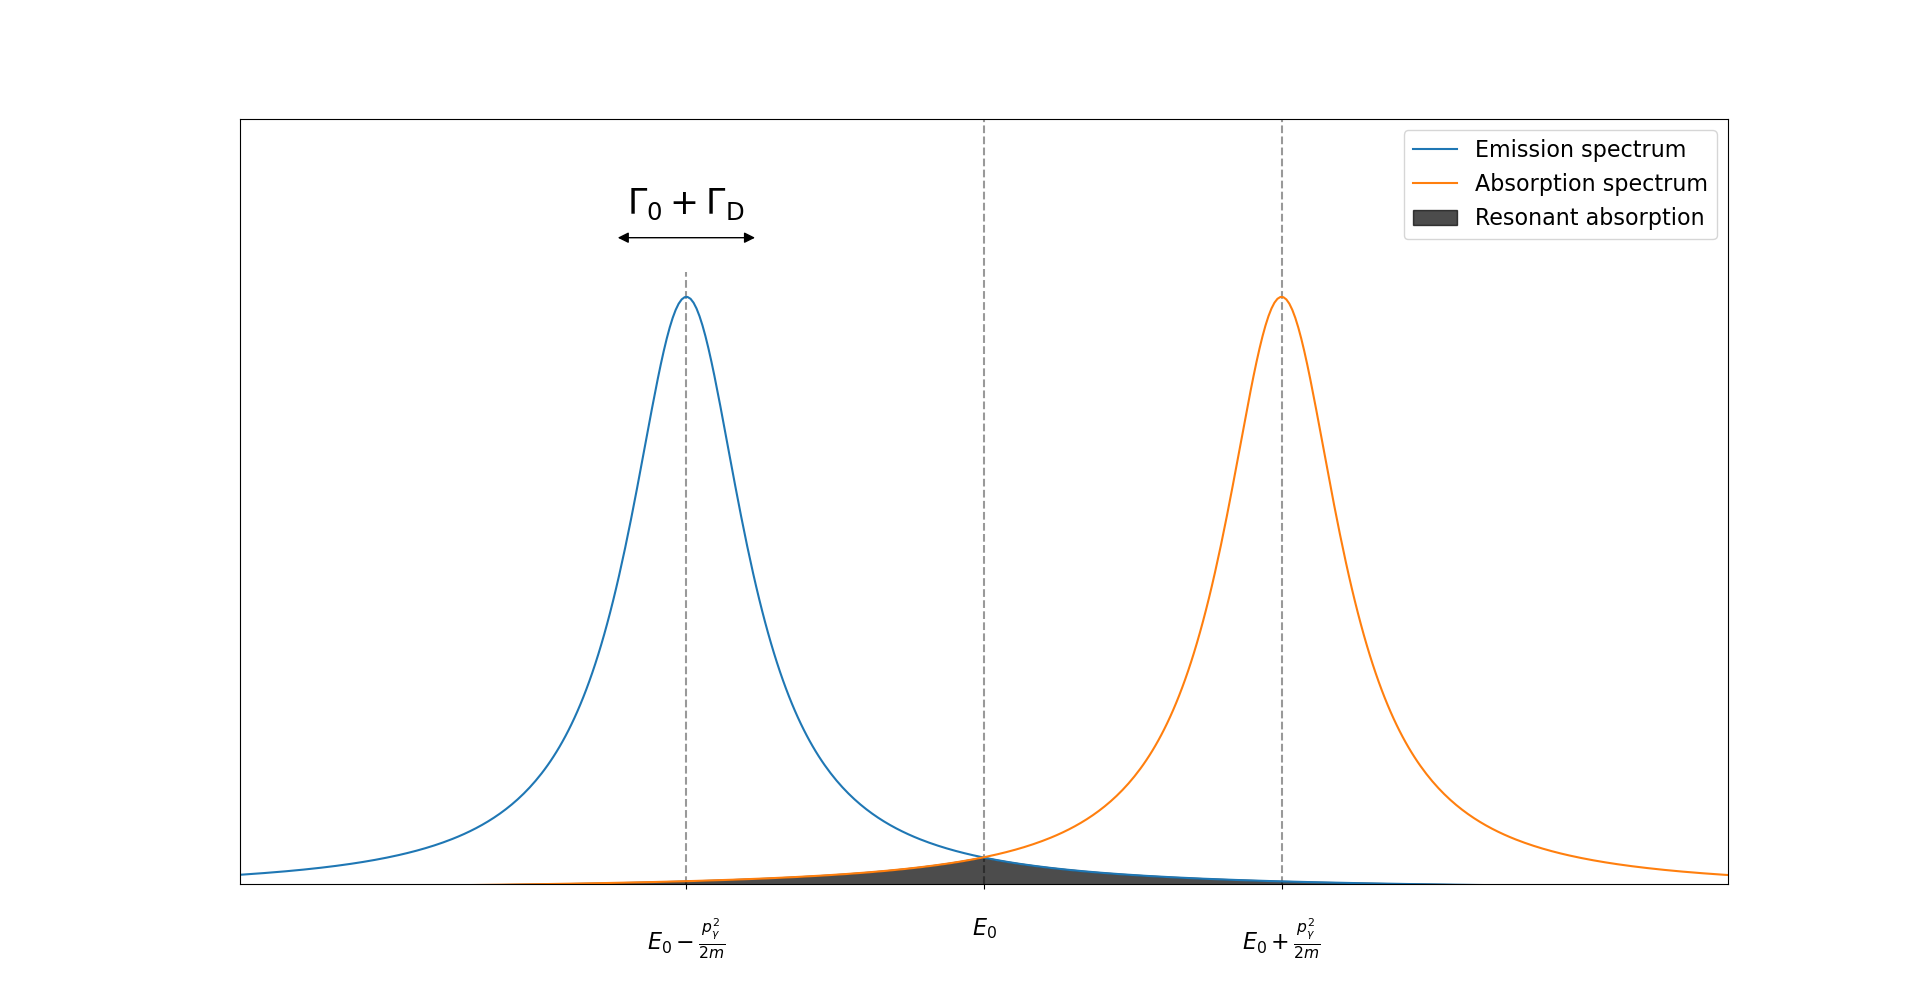
\includegraphics[height=4.0cm]{./fig/resonance-absorption-loose.png}
	\caption{\textbf{Natural + Doppler broadening}\label{fig:resonance-absorption-loose}}
	\end{subfigure}
	\caption{\textbf{(a)} The natural linewidth $\Gamma_0$ is not sufficient for
	a sizeable overlap of both spectra. Resonance absorption is not possible. 
	\textbf{(b)} The line width of both spectra can be increase by other effects 
	such as Doppler broadening. In such cases the spectra with linewidth 
	$\Gamma_0+\Gamma_\text{D}$ can overlap and resonant absorption is possible.
	\label{fig:resonant-absorption}}
\end{figure}

As it turns out, the above rules stating when resonant absorption can and cannot
occur are not strictly true. Experiments in the 1960s conducted by R. Mössbauer 
(\cite{wertheim2013mossbauer}) showed that resonant absorption in a crystal lattice
happens much more readily than one would expect based on the previous discussion.
The difference is the tight binding of the atoms in the crystal lattice. Instead of
the individual atom recoiling, different phonons can be created (or destroyed) by the
emission and absorption. In a sense, the entire crystal absorbs the recoil energy, 
effectively substituting the atom mass $m$ in equation \autoref{eq:energy-gap} by
the mass $M$ of the entire crystal. Because $m\ll M$, the energy gap between emission
and absorption spectrum drastically decreases. This phenomenon of recoilless nuclear
resonant absorption is named \textbf{Mössbauer effect}.
